% LM_C4-134-152 (scans 134-152), second pass: checked line by line against the scans; changes in LM_C4-134-152_changes.md
\scanpage{134}

\margin{\figure{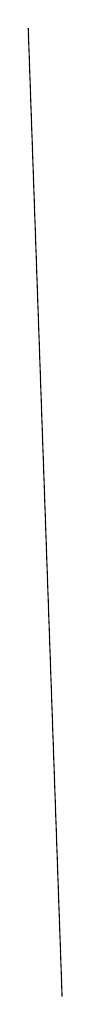
\begin{tikzpicture}\draw (0,0) -- (0.43,-12.3);\end{tikzpicture}}}

of $\mathcal M$ satisfying the following conditions

\par a) $M\longrightarrow\widetilde{\widetilde{\mathcal M}}$ (\unsure{composite} $M\longrightarrow\widetilde{\mathcal M}\longrightarrow\widetilde{\widetilde{\mathcal M}}$) is injective,

\par \deleted{b) $\unsure{\Gamma'}\ \widetilde{\widetilde{\mathcal M}}/\unsure{M|\Gamma}$}

\par hence extension

\par $(293)$\quad
\diagram{\begin{tikzcd}[ampersand replacement=\&,column sep=small]
1\arrow[r,dash]\&M\arrow[r,dash]\&\widetilde{\widetilde{\mathcal M}}\arrow[r,dash]\&\deleted{\unsure{\widetilde{\widetilde{\mathcal M}}/M}}\,\underset{\inserted{\overset{\mathrm{dfn}}{=}\widetilde{\widetilde{\mathcal M}}/M}}{\Gamma'}\arrow[r,dash]\&1
\end{tikzcd}}

\par b) \deleted{$\unsure{\widetilde{\widetilde{\mathcal M}}/M}$} $\Gamma'\overset{\mathrm{dfn}}{=}\widetilde{\widetilde{\mathcal M}}/M$ operates \uline{\unsure{faithfully}} on $M$,

\par i.e. we have
\[
\Gamma'\simeq\widetilde\Gamma=\operatorname{Im}(\Gamma\longrightarrow\operatorname{Aut}(M)).
\]

\par c) The extension $\widetilde{\widetilde{\mathcal M}}$ of $\Gamma'\simeq\widetilde\Gamma$ by $M$ is trivial (i.e. its class in $H^2(\widetilde\Gamma,M)$ is zero).

\par For such a quotient $\widetilde{\widetilde{\mathcal M}}$\inserted{ of $\widetilde{\mathcal M}$}, we recover $E$ as the set of all the splittings of the extension $\widetilde{\widetilde{\mathcal M}}$ of $\widetilde\Gamma$ by $M$, \deleted{\unsure{by|which}} on which we have $\widetilde{\mathcal M}$ operate via $\widetilde{\widetilde{\mathcal M}}$ by conjugation -- the restriction of this operation to $M\subset\widetilde{\mathcal M}$ makes $E$ an $E$-torsor (by hypothesis $(292)$).


Let us return again to the particular case that interests us. In the preceding number\textsuperscript{o} $(12^{\mathrm o})$ we verified the \deleted{\unsure{tr}} relations $(292)$, showing at the same time that this famous extension $G_{\rho,\widetilde\sigma}$ of $\widetilde\Gamma\simeq\unsure{\widehat{\mathbb Z}^{*}}\times\mathfrak S_3$ by $M^{\wedge}$ (denoted $M$ in the general considerations)

\margin{133}

% Archive printed footer (not manuscript):
% 133
% https://grothendieck.umontpellier.fr
% Université de Montpellier, UMR CNRS 5149, Case courrier 051, Place Eugène Bataillon
% 34095 Montpellier cedex 5 - France

\scanpage{135}
\mspage{715}

was trivial, and that two splittings were conjugate by an element of $M$ and only one (it is this second assertion of existence and uniqueness of conjugation that is the geometric content of $(292)$).
Moreover, we have \deleted{\unsure{thus}} indeed constructed, in number\textsuperscript{o} $11$, a surjective homomorphism
\diagram{\begin{tikzcd}[ampersand replacement=\&]
\mathcal M=\mathcal M_{0,3}\arrow[r]\&G_{\rho,\widetilde\sigma}
\end{tikzcd}}
thus making $G_{\rho,\widetilde\sigma}$ a quotient of $\mathcal M$ and even of $\widetilde{\mathcal M}$, which has the properties a) b) c) of the preceding corollary. \uline{This therefore defines for us, up to unique isomorphism, an object of the category of} $\mathcal X'$,
\deleted{i.e. a pro-covering of}
\uline{or what amounts to the same, a pro-étale covering of} $(U_{0,3\,\mathbb Q},\mathfrak S_3)\unsure{\simeq}M'_{1,1\,\mathbb Q}$,
\uline{which after \deleted{extension}\inserted{forgetting} \unsure{the operations} of} $\mathfrak S_3$ \uline{and extension of the base from} $\mathbb Q$ \uline{to} $\overline{\mathbb Q}$, \uline{becomes the universal abelian covering of} $U_{0,3\,\overline{\mathbb Q}}$.

But on the other hand the tower of Fermat coverings provides us with quite exactly such an object -- and if

\margin{134}

% Archive printed footer (not manuscript):
% 134
% https://grothendieck.umontpellier.fr
% Université de Montpellier, UMR CNRS 5149, Case courrier 051, Place Eugène Bataillon
% 34095 Montpellier cedex 5 - France

\scanpage{136}

I had not had this Fermat tower at my disposal, I certainly would not have suspected that \deleted{\unsure{$\widetilde{\widetilde{\mathcal M}}$ extension|even this extension}} subextension $\mathfrak S^{+\wedge}/\mu_{\mathfrak S}$\inserted{$=\widetilde{\mathfrak S}^{+\wedge}$} \deleted{of $\unsure{H}$} of $\widetilde H^+\simeq\mathfrak S_3$ by $M^{\wedge}$ was split!

\margin{\figure{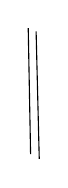
\begin{tikzpicture}\draw (0,0) -- (0.03,-1.6);\draw (0.10,-0.04) -- (0.14,-1.66);\end{tikzpicture}}}
The conjecture that presents itself at once is that these two pro-étale coverings are isomorphic -- the isomorphism between the two \unsure{is} then unique.


\deleted{\unsure{And}} This is the moment to determine the isomorphism classes of the \unsure{classes} of splittings of \inserted{the extension $\widetilde{\mathcal M}\unsure{\simeq}\mathcal M_{0,3}/[\widehat\Pi_{0,3},\widehat\Pi_{0,3}]$ of} $\Gamma=\Gamma_{\mathbb Q}\times\mathfrak S_3$ by $M^{\wedge}$, we have by the exact sequence associated with the Hochschild spectral sequence

$(294)$\quad
\diagram{\begin{tikzcd}[ampersand replacement=\&,column sep=small]
0\arrow[r,dash]\&H^1(\Gamma_{\mathbb Q},H^0(\deleted{\unsure{\widetilde\Gamma}}\mathfrak S_3,\widehat M))\arrow[r,dash]\&H^1(\unsure{\Gamma},\widehat M)\arrow[r,dash]\&H^0(\Gamma_{\mathbb Q},H^1(\mathfrak S_3,\widehat M))\arrow[d]\\
\&\&\&H^2(\Gamma_{\mathbb Q},H^0(\mathfrak S_3,M))
\end{tikzcd}}

Now we have seen that
\[
(295)\qquad H^0(\mathfrak S_3,\widehat M)=0
\qquad(\text{\unsure{and} }\overline{\mathrm m}\ H^0(\unsure{L_\rho|L_j},\unsure{\widehat M|\overline M})=0)
\]
\margin{hence $H^1(\Gamma,\widehat M)\simeq H^0(\Gamma_{\mathbb Q},H^1(\mathfrak S_3,\widehat M))$}
\deleted{\unsure{And}} Let us compute on the other hand
\[
H^1(\mathfrak S_3,\widehat M)=H^1(\mathfrak S_3,M)\otimes_{\mathbb Z}\widehat{\mathbb Z},
\]

\margin{135}

% Archive printed footer (not manuscript):
% 135
% https://grothendieck.umontpellier.fr
% Université de Montpellier, UMR CNRS 5149, Case courrier 051, Place Eugène Bataillon
% 34095 Montpellier cedex 5 - France

\scanpage{137}
\mspage{716}

which \unsure{returns} us to computing
\[
H^1(\mathfrak S_3,M)\quad ?
\]
But the study made of the extension $\mathfrak S^+/\mu_{\mathfrak S}$ of $\mathfrak S_3$ by $M$ -- which has shown us that this extension was split, and that two splittings were conjugate by a unique element of $M$, gives us in fact
\[
(296)\qquad
\left\{\begin{array}{ll}
H^0(\mathfrak S_3,M)=H^1(\mathfrak S_3,M)=0&\text{hence}\\
H^0(\mathfrak S_3,\unsure{\widehat M|\overline M})=H^1(\mathfrak S_3,\unsure{\widehat M|\overline M})=0&
\end{array}\right.
,
\]
hence finally, thanks to $(295)$, the triumphant relation
\[
(297)\qquad\boxed{H^1(\Gamma_{\mathbb Q}\times\mathfrak S_3,\widehat M)=0}\qquad !
\]

We thus find -- once again against all expectations, I confess! -- the

\uline{Theorem}\quad There exists a pro-étale \deleted{pro}covering
\margin{\figure{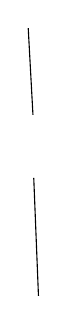
\begin{tikzpicture}\draw (0,0) -- (0.06,-1.1);\draw (0.07,-1.9) -- (0.13,-3.4);\end{tikzpicture}}}
\deleted{$\unsure{X|Z}$} $U_\infty$ of $(U_{0,3\,\mathbb Q},\mathfrak S_3)$\inserted{$=M'_{1,1\,\mathbb Q}$}, having the following property: The inverse image \inserted{$\overline U_\infty$} of $U_\infty$ over $U_{0,3\,\overline{\mathbb Q}}$ (\deleted{\unsure{without}}\inserted{\unsure{forgetting}} operations of $\mathfrak S_3$) is ``the'' universal abelian covering of $U_{0,3\,\overline{\mathbb Q}}$. For two such cover-

\margin{136}

% Archive printed footer (not manuscript):
% 136
% https://grothendieck.umontpellier.fr
% Université de Montpellier, UMR CNRS 5149, Case courrier 051, Place Eugène Bataillon
% 34095 Montpellier cedex 5 - France

\scanpage{138}

ings pro-étale over $(U_{0,3\,\mathbb Q},\mathfrak S_3)=M'_{1,1\,\mathbb Q}$, there exists a unique isomorphism from one onto the other.

We have obtained existence in \uline{two} ways: by the Fermat tower, and by the general theory of \S\,$49$ \uline{III}, applied to the present case -- which gives us a $U_\infty$ and a $U'_\infty$, each described up to unique isomorphism! The uniqueness theorem follows from the preceding little calculation -- I was afraid of the ``big'' \deleted{$\unsure{H^1(\Gamma_{\mathbb Q},\widehat M)\simeq H^1(\Gamma}$}
\[
H^1(\Gamma_{\mathbb Q},\widehat M)\simeq
M\otimes_{\mathbb Z}\underbrace{H^1(\Gamma_{\mathbb Q},T_{\unsure{\infty|*}}(G_m))}_{\widehat{\mathbb Q^{*}}},
\]
but in the end it is the vanishing of $H^{i}(\mathfrak S_3,M)$ for $i=0,1$ that implies (without knowing anything about $\Gamma_{\mathbb Q}$!) that of $H^1(\Gamma_{\mathbb Q}\times\mathfrak S_3,\widehat M)$, which ensures the uniqueness we needed.

\margin{137}

% Archive printed footer (not manuscript):
% 137
% https://grothendieck.umontpellier.fr
% Université de Montpellier, UMR CNRS 5149, Case courrier 051, Place Eugène Bataillon
% 34095 Montpellier cedex 5 - France

\scanpage{139}
\mspage{717}

\deleted{For} The preceding theorem completely elucidates, it seems to me, the arithmetico-geometric meaning (in terms of the Fermat tower) of the homomorphism ((218) page~695')
\[
\mathcal M=N_{1,1}^{\text{ét}}\longrightarrow G_{\rho,\sigma}\simeq\widehat{\mathbb Z}^{*}\mathbin{.}\mathfrak S_{\unsure{\bullet|0}}^{+\wedge}
\]
obtained in section 11°) by purely algebraic means --- or at least that of the slightly weaker homomorphism
\[
\mathcal M\longrightarrow\overbrace{G_{\rho,\sigma}/\mu_{\mathfrak S}}^{\inserted{G_{\rho,\widetilde{\sigma}}\overset{\mathrm{dfn}}{=}}}\simeq\widehat{\mathbb Z}^{*}\mathbin{.}\mathfrak S^{+\wedge}/\mu_{\mathfrak S}
\]
which factors \deleted{through} into a homomorphism
\[
\underbrace{\widetilde{\mathcal M}}_{\inserted{\text{denoted }\mathcal M\text{ in the preceding pages}}}\overset{\mathrm{dfn}}{=}\mathcal M/(\mu_{\mathcal M}=\mu_{\mathfrak S_{\unsure{0|\bullet}}})\longrightarrow G_{\rho,\widetilde{\sigma}}
\qquad\text{extension of }\widetilde\Gamma=\widehat{\mathbb Z}^{*}\times\mathfrak S_3\text{ by }M^\wedge.
\]

The passage from $G_{\rho,\sigma}^{\deleted{\unsure{\sim}}}$ to $G_{\rho,\widetilde{\sigma}}$, from the present point of view, had as its essential role (a posteriori!) to provide an extension by $M^\wedge$ (playing the role of an identity component) of a group operating \uline{faithfully} on $M^\wedge$, which was not the case for the extension $G_{\rho,\sigma}$ of $\widehat{\mathbb Z}^{*}\times H^+$ by $M^\wedge$, since the \deleted{\unsure{center|element}} \inserted{center $\mu_{H^+}=\{1,\unsure{\omega_{H^+}}\}$ \deleted{\unsure{$H^+$}} of $H^+$} operated trivially.
\margin{138}

% Archive printed footer (not manuscript):
% 138
% https://grothendieck.umontpellier.fr
% Université de Montpellier, UMR CNRS 5149, Case courrier 051, Place Eugène Bataillon
% 34095 Montpellier cedex 5 - France

\scanpage{140}

This, together with the relations
\[
H^0(\widehat{\mathbb Z}^{*}\times\mathfrak S_3,\widehat M)=H^1(\widehat{\mathbb Z}^{*}\times\mathfrak S_3,\widehat M)=0,
\]
made it possible to interpret the group $G_{\rho,\widetilde\sigma}$ as a group of transformations on the set $E$ of its own splittings, which made it possible to interpret the homomorphism $\mathcal M\to G_{\rho,\widetilde\sigma}$ (or $\widetilde{\mathcal M}\to G_{\rho,\widetilde\sigma}$) as an \deleted{\unsure{ho}} \uline{operation} of $\mathcal M$ \deleted{\unsure{of $H$}} (or better, \deleted{of $\unsure{\widetilde{\mathcal M}}$}\inserted{of $\widetilde{\mathcal M}=\pi_1(U_{0,3\mathbb Q},\mathfrak S_3)=\pi_1(M'_{1,1\mathbb Q})$} on $E$), thus corresponding to a \inserted{pro-étale} covering of $(U_{0,3\mathbb Q},\mathfrak S_3)\simeq M'_{1,1\mathbb Q}$ --- and this covering is none other than the Fermat pro-covering.

It remained to interpret in an analogous way the homomorphism $\boxed{\mathcal M=N_{1,1}\longrightarrow G_{\rho,\sigma}}$, fitting into the homomorphism of exact sequences
\[
\tag{298}
\diagram{\begin{tikzcd}[ampersand replacement=\&,column sep=small,row sep=large]
1\arrow[r]\&\begin{gathered}\mu_{\mathcal M}\\\Vert\\(\{1,\omega\})\end{gathered}\arrow[r]\arrow[d,"\simeq"]\&\begin{gathered}\mathcal M\\\Vert\\(N_{1,1})\end{gathered}\arrow[r]\arrow[d]\&\begin{gathered}\widetilde{\mathcal M}\\\Vert\\(N'_{1,1}=\unsure{\mathcal M_{0,3}})\end{gathered}\arrow[r]\arrow[d]\&1\\
1\arrow[r]\&\begin{gathered}\mu_G\\\Vert\\\{1,\omega\}\end{gathered}\arrow[r]\&G_{\rho,\sigma}\arrow[r]\&G_{\rho,\widetilde\sigma}\arrow[r]\&1
\end{tikzcd}},
\]
\deleted{For} which moreover makes it possible to interpret $\mathcal M$, as a central extension of $\widetilde{\mathcal M}$
\margin{139}

% Archive printed footer (not manuscript):
% 139
% https://grothendieck.umontpellier.fr
% Université de Montpellier, UMR CNRS 5149, Case courrier 051, Place Eugène Bataillon
% 34095 Montpellier cedex 5 - France

\scanpage{141}
\mspage{718}

by $\mu$, as the inverse image of the extension $G_{\rho,\sigma}$ of $G_{\rho,\widetilde\sigma}$ by $\mu$, under the preceding homomorphism $\widetilde{\mathcal M}\to G_{\rho,\widetilde\sigma}$. There is a striking analogy with what had happened, moreover, when we had started \unsure{from} (in \S~48, and \unsure{in|of} certain developments which preceded it) from the quotient group (``of Lie type'') $\unsure{\mathrm{SL}(2,\widehat{\mathbb Z})'}$ of $\unsure{\mathfrak S_{0,3}^{+\wedge}}$, to construct a homomorphism
\[
\deleted{\unsure{\mathcal M}}\qquad \mathcal M_{0,3}\longrightarrow\mathrm{GL}(2,\widehat{\mathbb Z})/\{\pm1\}
\]
from which it was possible for us to reconstruct \deleted{$\unsure{\mathcal M}$} the extension $\mathcal M=N_{1,1}$ of $\mathcal M_{0,3}$ by $\mu$ precisely as the inverse image of the extension $\mathrm{GL}(2,\widehat{\mathbb Z})$ of $\mathrm{GL}(2,\widehat{\mathbb Z})/\{\pm1\}$ by $\mu=\{\pm1\}$. From the present point of view where I am trying to make arithmetic-geometric aspects as explicit as possible in terms of automorphisms of the \inserted{profinite} groups with loops $\Pi_{0,3}^\wedge$ --- the remarkable fact is that the two
\margin{140}

% Archive printed footer (not manuscript):
% 140
% https://grothendieck.umontpellier.fr
% Université de Montpellier, UMR CNRS 5149, Case courrier 051, Place Eugène Bataillon
% 34095 Montpellier cedex 5 - France

\scanpage{142}

extensions of $\widetilde{\mathcal M}$ by $\mu$, coming out of apparently rather different calculations, are canonically isomorphic.

I presume that a general explanation of this fact \unsure{will not present|would not present} any difficulty, in the present context --- because in both cases, the \inserted{bi-}\unsure{covering} of $\unsure{\mathrm{GL}|\mathrm{SL}}(2,\widehat{\mathbb Z})/\pm1$ resp. of $G_{\rho,\widetilde\sigma}$ came from the fact that I had started from a quotient group ($\mathrm{SL}(2,\widehat{\mathbb Z})$ or $\mathfrak S^{+\wedge}$) \uline{not} of $\mathfrak S_{0,3}^{+\wedge}\simeq\mathrm{SL}(2,\mathbb Z)^\wedge/\pm1$, but of $\mathrm{SL}(2,\mathbb Z)^\wedge\simeq N_{1,1}$ itself ---

If we nevertheless look for an interpretation (of the ``Fermat tower'' kind) of the homomorphism $\mathcal M\to G_{\rho,\sigma}$, it would be necessary to interpret $G_{\rho,\sigma}$ \inserted{(as \unsure{was} $G_{\rho,\widetilde\sigma}$)} as a group of automorphisms of a ``typical fiber'' ``not too big'' --- the difficulty being to invent something on which \unsure{that|it} operates nontrivially.
\margin{141}

% Archive printed footer (not manuscript):
% 141
% https://grothendieck.umontpellier.fr
% Université de Montpellier, UMR CNRS 5149, Case courrier 051, Place Eugène Bataillon
% 34095 Montpellier cedex 5 - France

\scanpage{143}
\mspage{719}

Interpreting $\mathcal M_{0,3}=N'_{1,1}$ as $\pi_1(M'_{1,1})$, where $M'_{1,1}$ is the modular scheme/$\mathbb Q$ of elliptic curves up to symmetry, we see that the Fermat tower amounts to this: over every base scheme $S$ (say \inserted{\uline{of characteristic 0}}) and \unsure{every|every} quasi-elliptic curve \inserted{\deleted{$\unsure{E}$}$\widetilde X$} over $S$, let us consider the corresponding étale covering of degree three $S'$ of $S$ (\inserted{of the} ``points of order 2 of $\widetilde X$''), \deleted{let us put} let
\[
\tag{299}
\deleted{\unsure{M_2}}\quad M_0(\widetilde X/\unsure{S|B})\overset{\mathrm{dfn}}{=}p_*(\mathbb Z_{\unsure{S'|B'}})/\mathbb Z_S
\]
be the corresponding twisted constant $\mathbb Z$-module free of rank \deleted{three}\inserted{two}, and let us consider
\[
\tag{300}
\deleted{\unsure{M_2}}\quad M_1(\widetilde X/S)\overset{\mathrm{dfn}}{=}M_0(\widetilde X/S)\otimes_{\mathbb Z}\underbrace{\unsure{\widehat{\mathbb Z}(1)}}_{\inserted{\begin{gathered}\Vert\,\mathrm{dfn}\\T_\infty(\mathbb G_m)\end{gathered}}},
\]
which is a pro-étale \deleted{pro}group over $S$, a system of coefficients locally isomorphic (in the broad sense) to $\widehat{\mathbb Z}^{2}$. \deleted{This being so,}\inserted{Of} course, $M_1(\widetilde X/S)$ depends \unsure{functorially} on $\widetilde X/S$ for isomorphisms and inverse images (we have a cartesian section of an ad-hoc fibered category $\ldots$). This being so,
\margin{142}

% Archive printed footer (not manuscript):
% 142
% https://grothendieck.umontpellier.fr
% Université de Montpellier, UMR CNRS 5149, Case courrier 051, Place Eugène Bataillon
% 34095 Montpellier cedex 5 - France

\scanpage{144}

giving the ``Fermat tower'' is equivalent to giving, for $\forall\,\widetilde X/S$ as above, a torsor
\[
\tag{301}
F_\infty(\widetilde X/S)\quad\text{torsor over }S\text{ under }M_1(\widetilde X/S),
\]
\margin{for a geometric construction cf. (320) page 724}
compatible with isomorphisms and \unsure{changes} of base.

The preceding theorem says essentially that such an $F_\infty(\widetilde X/S)$ exists, and is unique up to unique isomorphism, requiring in addition that the natural homomorphism
\diagram{\begin{tikzcd}[ampersand replacement=\&]
\Pi_{0,3}^{\wedge}\arrow[r] \& M^{\wedge}
\end{tikzcd}}
associated with such a datum $F_\infty$ be the canonical homomorphism $\ldots$.

On the other hand, let $X$ be a relative elliptic curve over a base $S$ of characteristic 0, and let $S'\subset X$ be the closed subscheme, étale of degree 3 over $S$, corresponding to the points of order 2. Let us consider the \unsure{generalized Jacobian} of $X$ deduced from this multisection, let $\mathcal J^0$ be its part of degree 0, we thus have

\margin{143}

% Archive printed footer (not manuscript):
% 143
% https://grothendieck.umontpellier.fr
% Université de Montpellier, UMR CNRS 5149, Case courrier 051, Place Eugène Bataillon
% 34095 Montpellier cedex 5 - France

\scanpage{145}
\mspage{720}

an exact sequence
\[
\tag{302}
\diagram{\begin{tikzcd}[ampersand replacement=\&]
1\arrow[r] \& \mathcal J_0^0\arrow[r,dash]\arrow[d,phantom,"\rotatebox{90}{$\simeq$}" description] \& \mathcal J^0\arrow[r] \& X\arrow[r,dash] \& 1\\
\& \mathbb G_m\otimes_{\mathbb Z}M_0
\end{tikzcd}}
\]
where $M_0=M_0(X/S)$ is defined above (299). From this we deduce an exact sequence
\[
\tag{303}
\diagram{\begin{tikzcd}[ampersand replacement=\&]
1\arrow[r] \& M_1\arrow[r]\arrow[d,equal] \& T_\infty(\mathcal J^0)\arrow[r] \& T_\infty(X)\arrow[r,dash] \& 1\\
\& M_0\otimes_{\mathbb Z}T_\infty(\mathbb G_m)
\end{tikzcd}}
\]
where
\[
\tag{\uline{304}}
T_\infty(G)=\varprojlim_n {}_nG
\]
is the local system of the $\Pi_1$ of the smooth commutative group scheme \inserted{with connected fibers} over $S$. Thus giving a torsor under $M_1$ is equivalent to giving a torsor under $T_{\unsure{\infty|\alpha}}(\mathcal J^0)$, equipped with a section of the associated torsor \unsure{of the|of} group $T_\infty(X)$.
\unsure{Is there|Is there} a remarkable description of the Fermat torsor $F_\infty(X/S)$, in terms of the geometry of the relative elliptic curve $X/S$?

\margin{144}

% Archive printed footer (not manuscript):
% 144
% https://grothendieck.umontpellier.fr
% Université de Montpellier, UMR CNRS 5149, Case courrier 051, Place Eugène Bataillon
% 34095 Montpellier cedex 5 - France

\scanpage{146}

$14^\circ)$ Relation to generalized Jacobians.

Let us consider the ``generalized Jacobian'' of
\[
\inserted{U_{0,3}={}}U_{0,3\,\deleted{\unsure{\mathbb Q}}\inserted{\mathbb Z}}
=\deleted{\unsure{\mathbb A_{\mathbb Q}}}\mathbb P^1_{\deleted{\unsure{\mathbb Q}}\inserted{\mathbb Z}}
-\{0,1,\infty\}_{\deleted{\unsure{\mathbb Q}}\inserted{\mathbb Z}},
\]
it is thus a group scheme $\mathcal J^*_{U_{0,3}}=\mathcal J^*$, \unsure{augmented|mapping} to $\mathbb Z$, fitting into the exact sequence
\[
\tag{305}
\diagram{\begin{tikzcd}[ampersand replacement=\&]
1\arrow[r] \& \mathcal J^0\arrow[r]\arrow[d,phantom,"\rotatebox{90}{$\simeq$}" description] \& \mathcal J^*\arrow[r,"\deg"] \& \mathbb Z_{\inserted{S_0}\deleted{\unsure{\mathbb Q}}}\arrow[r] \& 1\\
\& \mathbb G_{mS_0}\otimes_{\mathbb Z}M_{\unsure{0|\mathbb Z}}
\end{tikzcd}},
\]
\margin{\uline{N.B.} $S_0\overset{\unsure{\mathrm{df}|\mathrm{dfn}}}{=}\operatorname{Spec}\mathbb Z$}
and equipped with a canonical \deleted{homo}morphism
\[
\tag{306}
\diagram{\begin{tikzcd}[ampersand replacement=\&]
\varphi:\ U_{0,3\,\deleted{\unsure{\mathbb Q}}\inserted{\mathbb Z}}\arrow[r] \&
\underbrace{\mathcal J^1}_{\substack{\text{subscheme of }\mathcal J^*\\\text{inverse image of}\\\text{the section }1\text{ of }\mathbb Z_{S_0}}}
\end{tikzcd}}
\]
The operations of $\mathfrak S_3$ on $U_{0,3}$ define by functoriality operations of $\mathfrak S_3$ on $\mathcal J^*$, compatible with the extension structure (305), and such that (306) commutes with the operations of $\mathfrak S_3$.
Let us note that $\mathcal J^1$ is a $\mathcal J^0$-torsor and

\margin{145}

% Archive printed footer (not manuscript):
% 145
% https://grothendieck.umontpellier.fr
% Université de Montpellier, UMR CNRS 5149, Case courrier 051, Place Eugène Bataillon
% 34095 Montpellier cedex 5 - France

\scanpage{147}
\mspage{721}

even an $(\mathfrak S_3,\mathcal J^0)$-torsor (a $\mathcal J^0$-torsor on which $\mathfrak S_3$ operates in a way compatible with its operations on $\mathcal J^0$), hence classified by an element of $H^1(S_0,\mathfrak S_3;\mathcal J^0)$. Now I presume that we have
\[
\tag{307}
H^0(S_0,\mathfrak S_3,\mathcal J^0)=H^1(S_0,\mathfrak S_3,\mathcal J^0)=0
\]
(where
\[
\tag{308}
\left\{\begin{aligned}
S_0&=\operatorname{Spec}\mathbb Z,\quad \mathcal J^0=\mathbb G_m\times_{\mathbb Z}M\simeq\mathbb G_m^{\{0,1,\infty\}}/\mathrm{diag}\\
&\simeq\operatorname{Ker}\left(\diagram{\begin{tikzcd}[ampersand replacement=\&,column sep=small]
\mathbb G_m^{\{0,1,\infty\}}\arrow[r] \& \mathbb G_m^{\deleted{\unsure{\{0,1,\infty\}}}}\\
(x_0,x_1,x_\infty)\arrow[r,mapsto] \& \substack{\inserted{x_0\cdot x_1\cdot x_\infty}\\\deleted{\unsure{(x_1x_\infty^{-1},x_\infty x_0^{-1},x_0x_1^{-1})}}}
\end{tikzcd}}\right)
\end{aligned}\right.
\]
\margin{Careful, this last isomorphism is obtained \unsure{via}
\diagram{\begin{tikzcd}[ampersand replacement=\&]
(x_0,x_1,x_\infty)\arrow[r,mapsto] \& (x_1x_\infty^{-1},x_\infty x_0^{-1},x_0x_1^{-1})
\end{tikzcd}}, which commutes with $\mathfrak S_3^+$, but \unsure{not|not} with $\mathfrak S_3$ as a whole}

We have indeed
\[
\begin{aligned}
H^0(S_0,\mathfrak S_3;\mathcal J^0)&\simeq\left\{(x_0,x_1,x_\infty)\in\mathbb Z^{*\{0,1,\infty\}}\ \middle|\ \begin{array}{l}x_0x_1x_\infty=1\\(x_0,x_1,x_\infty)\text{ invariant under }\mathfrak S_3\end{array}\right\}\\
&=\{(x,x,x)\mid x\in\mathbb Z^{*\{0,1,\infty\}},\quad x^3=1\}\\
&=1
\end{aligned}
\]
\margin{Calculation \unsure{correct}, for it \unsure{rests on this} $\mathfrak S_3^+$-isomorphism which is not an $\mathfrak S_3$-isomorphism, \unsure{it seems here to be|there seems not to be} need of $H^0(S,\mu_3)=1$, whereas a calculation already made of the \unsure{splittings} of extensions (cf. 720) shows that $\unsure{S}$ -- over \uline{any} \uuline{base}
\diagram{\begin{tikzcd}[ampersand replacement=\&,column sep=small]
H^0(S,\mathfrak S_3,\mathcal J^0)\arrow[d,equal]\arrow[r,phantom,"\simeq"] \& H^1(\deleted{\unsure{S,}}\mathfrak S_3;H^0(\unsure{S|S_0},\mathcal J^0))\simeq0\quad\unsure{\Leftarrow}\\
H^0(\mathfrak S_3,H^0(S,\mathcal J^0))
\end{tikzcd}}}

(\unsure{the} only cube \deleted{\unsure{of}} root of 1 in $\mathbb Z$ (or even in $\mathbb Q$) is 1. This establishes the first relation (307). For the second, we use the spectral sequence

\margin{146}

% Archive printed footer (not manuscript):
% 146
% https://grothendieck.umontpellier.fr
% Université de Montpellier, UMR CNRS 5149, Case courrier 051, Place Eugène Bataillon
% 34095 Montpellier cedex 5 - France

\scanpage{148}

\diagram{\begin{tikzcd}[ampersand replacement=\&]
H^{\unsure{*|n}}(S_0,\mathfrak S_3;\mathcal J^0) \&
\overset{\inserted{E_2^{pq}=}}{H^p(\mathfrak S_3,\uline{H}^{q}(S_0,\mathcal J^0))}\arrow[l,Rightarrow]
\end{tikzcd}}
which gives the exact sequence
\diagram{\begin{tikzcd}[ampersand replacement=\&,column sep=small]
0\arrow[r] \& H^1(\mathfrak S_3,H^0(S_0,\mathcal J^0))\arrow[r,"\unsure{\deleted{\simeq}|\simeq}"] \& H^1(S_0,\mathfrak S_3;\mathcal J^0)\arrow[r] \& H^0(\mathfrak S_3,H^1(S_0,\mathcal J^0))\arrow[d]\arrow[dl,equal]\\
\& \& \bigl(H^{\unsure{0|q}}(\mathfrak S_3,M_{\unsure{0}}\otimes_{\mathbb Z}H^1(S_0,\mathbb G_m))\bigr) \& H^2(\mathfrak S_3,H^0(S_0,\mathcal J^0))
\end{tikzcd}}

Now we have
\[
H^1(S_0,\mathcal J^0)\simeq H^1(S_0,\mathbb G_m^2)\simeq\operatorname{Pic}(\unsure{S|S_0})^2=0
\]
\margin{\uline{N.B.} we do \uline{not} need the relation $\operatorname{Pic}(S)=0$}
hence we get
\[
H^1(S_0,\mathfrak S_3;\mathcal J^0)\simeq H^1(\mathfrak S_3,\underbrace{H^0(S_0,\mathcal J^0)}_{\substack{\deleted{(\mathbb Z^*)^{\{0,1,\infty\}}/\mathbb Z^*}\\\deleted{\simeq\mathbb Z^*\otimes_{\mathbb Z}M_0}}})
\]

But in fact, the calculations made elsewhere show that we have
\[
\tag{309}
H^0(\mathfrak S_3,M_{\unsure{0|\alpha}}\otimes_{\mathbb Z}\unsure{I|I_0})=H^1(\mathfrak S_3,M_{\unsure{0|\alpha}}\otimes_{\mathbb Z}I)=0
\]
for any $\mathbb Z$-module $I$ (for example $I=\unsure{J^0|\mathcal J^0}(S)$, $S$ an \unsure{arbitrary|arbitrary} scheme, \inserted{or $I=H^1(S,\mathbb G_m)=\operatorname{Pic}(S)$}), whence finally,
\[
\tag{\unsure{310}}
H^0(\unsure{\deleted{S_0}|S},\mathfrak S_3;\mathcal J^0)\simeq H^1(S,\mathfrak S_3,\mathcal J^0)=0
\]
for $\forall$ scheme $S$. We thus find:

\margin{147}

% Archive printed footer (not manuscript):
% 147
% https://grothendieck.umontpellier.fr
% Université de Montpellier, UMR CNRS 5149, Case courrier 051, Place Eugène Bataillon
% 34095 Montpellier cedex 5 - France

\scanpage{149}
\mspage{722}

\uline{Proposition} Let \deleted{$\unsure{\mathcal J}$}
$\mathcal J^0=\mathbb G_m^{\{0,1,\infty\}}/\underbrace{\mathbb G_m}_{\mathrm{diag.}}\simeq\mathbb G_m\otimes_{\mathbb Z}\unsure{M_0|M}$
Then for $\forall$ $(\mathfrak S_3,\mathcal J^0)$-torsor over an arbitrary base $S$, there exists a unique trivialization of it, i.e. a unique section, invariant under the operations of $\mathfrak S_3$.

\uline{Corollary 1} Over any base $S$, there exists a unique morphism
\[
(311)\qquad
\diagram{\begin{tikzcd}[ampersand replacement=\&]
\psi:U_{0,3\,S} \arrow[r] \& \mathcal J^0_S
\end{tikzcd}}
\]
which is compatible with the operations of $\mathfrak S_3$, and which (via the homomorphism
$\mathcal J^*_S\longrightarrow\mathcal J^0_S$ \unsure{which|that} \unsure{it|it} \unsure{is factored by}, by the universal property of the \illegible{1} generalized \unsure{Jacobians}) induces the identity homomorphism
$\underset{\inserted{\mathcal J^*_S}}{\mathcal J^0_S}-\mathcal J^0_S$.

\margin{\uline{N.B.} With the notation of \unsure{695}, we have $U_{0,3\,S}\simeq(U_1)_S$, where $U_1\subset\mathbb G_m^3/\mathbb G_m$ is \unsure{defined} by
\[
(312)\qquad
U_1=\{(x_0,x_1,x_\infty)\in\Gamma\mathbb G_m^{\{0,1,\infty\}}\mid x_0+x_1+x_\infty=\unsure{0}\}
\quad\mathrm{mod}\ \mathrm{diag}_3\mathbb G_m.
\]}

\uline{Corollary 3} Let $Y$ be a scheme of

\margin{148}

% Archive printed footer (not manuscript):
% 148
% https://grothendieck.umontpellier.fr
% Université de Montpellier, UMR CNRS 5149, Case courrier 051, Place Eugène Bataillon
% 34095 Montpellier cedex 5 - France

\scanpage{150}

\unsure{Brauer}-Severi over $S$, of relative dimension $1$ (i.e. a form of $\mathbb P^1_S$), equipped with a \inserted{closed} subscheme $S'\subset Y$, étale of degree $3$ over $S$, and let \deleted{$\unsure{X}$} $U=Y\setminus S'$, $\mathcal J^*_{U/S}$ the generalized Jacobian, so that we have
\[
(313)\qquad
\diagram{\begin{tikzcd}[ampersand replacement=\&,column sep=1.5em,row sep=.5em]
1 \arrow[r,no head] \& \mathcal J^0_{U/S} \arrow[r,no head] \arrow[d,phantom,"\unsure{\wr}" description] \& \mathcal J^*_{U/S} \arrow[r,no head] \& \mathbb Z_S \arrow[r,no head] \& 1 \\
\& \mathbb G_m\otimes_{\mathbb Z}\unsure{M_0}(S'/S) \& \& \&
\end{tikzcd}}
\]
where $\unsure{M_0}(S'/S)\simeq\unsure{p_*|\rho_*}(\mathbb Z_{S'})/\underbrace{\mathbb Z_S}_{\mathrm{diag}}$ is the $S$-scheme \inserted{of \deleted{groups} \inserted{$\mathbb Z$-modules}} (locally $\unsure{\overline{\mathrm{isom.}}}$ to $\mathbb Z^{\unsure{2}}$, deduced from $\unsure{M_{0\,S}}$ by twisting it (via the action of $\mathfrak S_3$) by the \deleted{principal bundle} \inserted{$\mathfrak S_3$-torsor over $S$} associated with $S'$.

There exists then a unique morphism
\[
(\unsure{314})\qquad
\diagram{\begin{tikzcd}[ampersand replacement=\&]
\psi:U \arrow[r] \& \mathcal J^0_{U/S}
\end{tikzcd}}
\]
commuting with \deleted{$\uline{\operatorname{Aut}}$} the action of $\uline{\operatorname{Aut}}(S'/S)\xleftarrow{\sim}\uline{\operatorname{Aut}}_S(Y,S')$, and inducing (by the universal property) \deleted{\unsure{a}} the \unsure{composite} homomorphism
\[
\diagram{\begin{tikzcd}[ampersand replacement=\&]
\mathcal J^0_{U/S} \arrow[r,hook] \& \mathcal J^*_{U/S} \arrow[r,"\widetilde\psi"] \& \mathcal J^0_{U/S}
\end{tikzcd}}
\]
which is the identity.

\margin{149}

% Archive printed footer (not manuscript):
% 149
% https://grothendieck.umontpellier.fr
% Université de Montpellier, UMR CNRS 5149, Case courrier 051, Place Eugène Bataillon
% 34095 Montpellier cedex 5 - France

\scanpage{151}
\mspage{723}

Let us make explicit \unsure{the|the} \deleted{homo}morphism
\[
(315)\qquad
\diagram{\begin{tikzcd}[ampersand replacement=\&,column sep=2em,row sep=.9em]
U_{0,3}=\mathbb P^1\setminus\{0,1,\infty\}_{S_0}
  \arrow[r,hook,"\psi"] \arrow[d,equal]
\& \underbrace{\mathbb G_m^{\{0,1,\infty\}}/\mathbb G_m}_{\unsure{\mathcal J^0}}
\\
\begin{gathered}
\deleted{\{z\in\unsure{\Gamma}\mathbb G_m\mid z-1\ \mathrm{inv}\}}\\
\unsure{(}\mathbb G_m\setminus\{1\}\unsure{)}_{S_0}
\simeq\{z\in\Gamma\mathbb G_m\mid z-1\ \mathrm{inv}\}
\end{gathered}
\& \begin{gathered}
\deleted{\unsure{\mathcal J^1}}\inserted{U_1=\{(x_0,x_1,x_\infty)^{\deleted{\unsure{\mathbb Z}}}
\in\Gamma\mathbb G_m^3/\mathbb G_m\mid}\\
\inserted{x_0+x_1+x_\infty=0\}}
\end{gathered} \arrow[u,hook]
\end{tikzcd}}
\]
\deleted{\unsure{it}} \deleted{\unsure{it is}} isomorphism of $U_{0,3}$ with $U_1$ which \deleted{\unsure{is}} corresponds: \deleted{\unsure{one must|extends}}
\[
(316)\qquad
\left\{\begin{array}{l}
\diagram{\begin{tikzcd}[ampersand replacement=\&,column sep=2em,row sep=.5em]
\overline\psi:\unsure{\widehat U_{0,3}|\overline U_{0,3}} \arrow[r] \arrow[d,equal]
\& \widehat U_1\subset\mathbb P^2_{S_0} \arrow[d,equal]\\
\mathbb P^1_{S_0}
\& \{(x_0,x_1,x_\infty)\in\unsure{\widehat{\mathbb P}^2_{\unsure{S_0}}|\mathbb P^2_{S_0}}\mid x_0+x_1+x_\infty=0\}
\end{tikzcd}}\\[1em]
\overline\psi(0)=(0,1,-1)\\
\overline\psi(1)=(-1,0,1)\\
\overline\psi(\infty)=(1,-1,0)
\end{array}\right.\ ,
\]
it suffices to take
\[
(317)\qquad
\psi(z)=(-z,z-1,1)=(1,1/z-1,-1/z)
\inserted{=\left(\frac{-z}{z-1},1,\frac{1}{z-1}\right)}.
\]

Let us now return to the datum of a relative elliptic curve \inserted{$X$} over $S$ modulo symmetry (corresponding to a morphism
$S\longrightarrow\deleted{\unsure{\operatorname{Spec}}}\mathcal M'_{1,1}$).

\margin{150}

% Archive printed footer (not manuscript):
% 150
% https://grothendieck.umontpellier.fr
% Université de Montpellier, UMR CNRS 5149, Case courrier 051, Place Eugène Bataillon
% 34095 Montpellier cedex 5 - France

\scanpage{152}

We assume $2$ invertible on $S$, so that the datum of $X$ \inserted{modulo $\omega_X$} corresponds, by the Legendre \unsure{carpet} $X\mapsto(X/\deleted{\text{\unsure{modulo symmetry}}}\inserted{\{1,\omega_X\}})$, to the datum of a $(Y,S')$ as above, with in \uline{addition} a section of $U=Y-S'$.

In fact, the datum of $(Y,S')$ amounts to the datum of $S'$, \inserted{i.e. of an $\mathfrak S_3$-torsor} \deleted{$Y$ is recovered} $T$ over $S$ --- and $Y$ is recovered from \unsure{there|it} as the twisted scheme $T\wedge_{\mathfrak S_3}\mathbb P^1_S$ \deleted{$\unsure{\wedge_{\mathfrak S_3}}$ \unsure{and|or}, $T\wedge_{\mathfrak S_3}\mathcal J^0_{(U_{0,3})_S}\simeq\unsure{\mathcal J^0}$}
with
\[
U=Y\setminus S'\simeq(T\wedge_{\mathfrak S_3}\mathbb P^1_S)\setminus\underbrace{T\wedge_{\mathfrak S_3}\{0,1,\infty\}_S}_{S'}
\]
canonically embedded in
\[
T\wedge_{\mathfrak S_3}\mathcal J^0_{(U_{0,3})_S}\simeq\mathcal J^0_{U/S}.
\]
The embedding $U\subset\mathcal J^0_{U/S}$ can also be interpreted as a canonical morphism
\[
(318)\qquad
\diagram{\begin{tikzcd}[ampersand replacement=\&]
X \arrow[r] \& \mathcal J^0_{U/S}\underbrace{=\unsure{\mathcal J^0_{0\,X/S}|\mathcal J^0_{X/S}}}_{\substack{\text{\unsure{with|in} notation}\\\text{of page }720}}
\end{tikzcd}}
\]
which should be easy to characterize \unsure{axiomatically}

\margin{151}

% Archive printed footer (not manuscript):
% 151
% https://grothendieck.umontpellier.fr
% Université de Montpellier, UMR CNRS 5149, Case courrier 051, Place Eugène Bataillon
% 34095 Montpellier cedex 5 - France
